\documentclass[11pt]{article} % use larger type; default would be 10pt
\usepackage[utf8]{inputenc} % set input encoding (not needed with XeLaTeX)

%%% BEGIN Article customizations

%%% PAGE LAYOUT
\usepackage{geometry} % to change the page dimensions
\geometry{a4paper} % or letterpaper (US) or a5paper or....
% \geometry{margin=1in} % for example, change the margins to 2 inches all round
\usepackage[parfill]{parskip} % Activate to begin paragraphs with an empty line rather than an indent

%%% FIGURES
\usepackage{graphicx} % support the \includegraphics command and options
\graphicspath{{../FIGURES/FIGURE_PDFS/}}

%%% PACKAGES
\usepackage{booktabs} % for much better looking tables
\usepackage{array} % for better arrays (eg matrices) in maths
\usepackage{paralist} % very flexible & customisable lists (eg. enumerate/itemize, etc.)
\usepackage{verbatim} % adds environment for commenting out blocks of text & for better verbatim
\usepackage{subfig} % make it possible to include more than one captioned figure/table in a single float
\usepackage{lscape}
% These packages are all incorporated in the memoir class to one degree or another...

%%% HEADERS & FOOTERS
\usepackage{fancyhdr} % This should be set AFTER setting up the page geometry
\pagestyle{fancy} % options: empty , plain , fancy
\renewcommand{\headrulewidth}{0pt} % customise the layout...
\lhead{}\chead{}\rhead{}
\lfoot{}\cfoot{\thepage}\rfoot{}

%%% SECTION TITLE APPEARANCE
\usepackage{sectsty}
\allsectionsfont{\sffamily\mdseries\upshape} % (See the fntguide.pdf for font help)
% (This matches ConTeXt defaults)

%%% ToC (table of contents) APPEARANCE
\usepackage[nottoc,notlof,notlot]{tocbibind} % Put the bibliography in the ToC
\usepackage[titles,subfigure]{tocloft} % Alter the style of the Table of Contents
\renewcommand{\cftsecfont}{\rmfamily\mdseries\upshape}
\renewcommand{\cftsecpagefont}{\rmfamily\mdseries\upshape} % No bold!

%%% END Article customizations

%%% The "real" document content comes below...

\title{Reproducibility of SNP calling in multiple sequencing runs from single tumors}
\author{Dakota Z. Derryberry, Claus O. Wilke, Matthew C. Cowperthwaite} %**ask them about author order, I'm out of it...

\begin{document}
\maketitle

\section{Abstract}

%A) What system are you studying?
We examined 55 technical sequencing replicates of Glioblatoma multiforme (GBM) tumors from The Cancer Genome Atlas (TCGA). %Each replicate included the tumor sequenced once using standard whole exome sequencing with amplification, and once without amplification prior to creating a library.
%B) Why is it important?
In recent years, TCGA \cite{TCGA-GBM} and others in cancer genomics \cite{Parsons} have used large scale sequencing results of many tumors to identify drivers and essential cancer genes using a variety of computational analyses. However, very little is known about the reproducibility of this genomic data and, given the heterogeneity found in tumors, it could be quite low.  
%C) What is your research approach?
Wemeasured the extent of the overlap between two technical sequencing replicates from the same tumor (n=55), to find what proportion of mutations were reliably found between them, using strictly computational means. We further examined whether the raw data was improved or not, as measured by the extent of the overlap, using the SNP calling program SomaticSniper.  
%D) (optional) How is your research different from previous work?
%E) What are the results of your research?
We found that in the raw data, about half of the mutations found in one sequencing run can be found in the second. Interestingly, the size of the overlap varies by two orders of magnitude, between about 50 and 7000. Using a SNP caller, rather than improving the data, removes the overlap completely. This is because overlap is almost entirely composed of LOH, removed automatically by SomaticSniper, and SNPs with only a few reads cvering the alternate allele.
%F) What conclusions can we draw from these results?
We interpret these results to mean that, as expected, sequencing runs of tumors detect many false positives, and the number of these is increased by an amplification step prior to building a library. This tendency aside, the actual number of muations in different tumors of the same type (GBM) may vary by orders of magnitude. Finally, while verificaion of sequencing using PCR remains the gold standard, when SNP-calling using strictly computational means, SNP-callers may actually decrease the quality of results.

\section{Introduction}

%A) What is the general field of study?
Glioblastoma multiforme (GBM) is the most common and deadly primary brain tumor, with a median survival of 13.9 months and a 5-year survival of ~5\% \cite{TCGA-GBM-13}. Prognosis for patients with this disease remains poor despite significant research investment, due to the difficulty of surgical resection and the limited number of effective chemoteraputics. Like all cancers, GBM is an evolutionary disease caused by mutations and other alterations to normal glial cell lines. However, following substantial research efforts dedicated to identifying all of the mutations in an individual patient's tumor to try and identify causal variants, few precise causal elationships have been identified. There are likely many related causes for this failure, including but not limited to genomic heterogeneity in tumors, \cite{ValentineD}, the view that "GBM growth is driven by a signaling network with functional redundancy that permits adaptation" \cite{TCGA-GBM-13}, and imperfect computational methods. 
%B) What is the specific question of the research?
In this paper, we are interested in the third. We used technical sequencing replicates from 55 GBM tumors to look at the reproducbility of the raw data using a standard computational pipeline. Assuming that those mutations that appear in each of the technical replicates are true positives, and all others are false positives (which in fact may or may not be true), we want to see what proportion of mutations recovered are true positives, and whether or not the proportion is increased by SNP-calling methods designed to remove false positives.

%C) Why is (a) and/or (b) important?
The past six years have seen an explosion of data in cancer genomics, an effort led by TCGA, an archive of publicly-available data that includes sequencing of paired tumor-normal samples from a single patient for thousands of tumors. TCGA's glioblastoma dataset alone includes some 580 (and constantly growing) tumor-normal pairs. A varity of researchers in cancer genomics have used this data to discover which genes and pathways are mutated in GBM \cite{pathways}, discover different GBM subtypes \cite{subtypes}, and develop a variety of computational models to find GBM driver mutations \cite{drivers}. Despite this apparent success, most of the relationships discovered, though real, are small effects, and few of these innovations have been successfully translated into clinically useful results and techniques. Several possible factors likely contribute to this effect.
%D) What has previously been done in this area?
[NAME] showed that batch effects have a significant effect on large scale sequencing projects such as TCGA \cite{batch-effects}, and that eliminating this bias without collecting thousands more samples is virtually impossible. While TCGA may eventually do this, eliminating these effects at this time is impossible. Secondly, multiple groups have shown that tumors are highly genetically heterogeneous, and sampling a tumor only once cannot show the entirely of the mutational profile of the tumor \cite{ValentineD} \cite{hetero1} \cite{hetero2}. Third, several groups have shown that epigenetic factors, including methylation \cite{methylation-new}, chromatin remodeling \cite{chromatin}, and micro-RNAs \cite{microRNA}, may significantly effect tumor development and growth. 
%E) How does your research differ?
For all of these reasons, and likley more besides, we know that tumor sequencing is imperfect, and results based on it have to account for a significant amount of noisy data. In this paper, we attempt to look at how much noise (without regard to the theoretical source of it). We take 55 TCGA samples with technical replicates, and look at the similarity of the replicates. 
%F) (end with) a summary of the research described in this paper
We took data from 55 TCGA samples that were sequenced twice, once with the standard WGS protocol, and once with an additional amplification step before library prep, which we call the WGA protocol. We aligned the data and used the SNP-calling program SomaticSniper. Comparing the WGS and WGA results of these 55 samples, we find significant overlap (around 50\%), but as many differences, between technical sequencing replicates of the same sample. As expected, we found that the additional amplification step in the WGA protocol versus the WGS protocol added some mutations to the sample, so that on average these replicates had (i) more mutations, and (ii) a smaller percentage overlap. The number of mutations per sample varied by orders of magnitude, from under 100 to almost 10,000. We expected to see the quality of results (measured by the percentage overlap between technical replicates) decrease with increasing numbers of mutations, but found no correlation. We next looked at standard computational filters meant to increase the quality of the data. We found that to the contrary, employing these filters completely removed the overlap between replicates, and that two filters in particular, one for quality of the alternate allele read and one for loss of heterozygosity, removed most of this data. We conclude that the number of mutations in GBM tumors may be more variable tthan is generally supposed. Further, while nothing will ever beat the biolgical goldstandard of PCR for mutation verification, computational methods need to improve.

\section{Results}

\subsection{Unfiltered data}

% Experiment: size of overlap (figures 1 and 2)
%(a) a brief (one sentence to one paragraph) summary of what you did and why
%(b) a description of what you found carrying out this experiment
Next-generation sequencing is far from perfect; it produces errors at a rate of around XX per Mbp, and those errors are both predictable and not. Cancer sequencing, with highly heterogenous DNA targets from impure tissue samples, is possibly even mroe unreliable. Thus, we expect a high number of false positives in tumor sequencing. The gold-standard for determining a true somatic mutation from a germ line mutation or a sequencing error is to double check for the variant with PCR, but this is expensive, time consuming with so many samples, and often not available. To try and estimate an approximate rate of false positives, we first looked at the degree of overlap between technical replicates in GBM sequencing. For 55 GBM tumors, TCGA provides two sets of raw sequence data, one set captured with tthe standard whole exome sequencing methods (WGA) including an amplification of the DNA extracted from the tumor prior to library prep, and one using a protocol for large quantities of DNA that omits this amplification (WGS). Our assumption is that putative SNPs appearing in both technical replicates are more likely to be true positives than those appearing only in one replicate.

For each sample, we called mutations in both technical replicates and the pateint's blood sample using the same computational pipeline (see Figure 1 and Methods): we used CGHub to download TCGA bamfiles aligned to hg18, re-generated teh fastq files with picard, re-aligned the fastq files to hg19 with bwa, performed indel re-alignment and base recalibration with GATK, and finally called somatic mutaitons with SomaticSniper. We then analyzed the list of putative SNPs generated for each replicate by SomaticSniper, as well as the intersection, or overlap, of the two lists. We found that the number of mutations found in one replicate correlated strongly with the number of mutations found in the other, though as expected the WGA replicate, with the additional amplification step, had slightly more mutations (Figure 3). We further found that the overlap between the two samples, caclulated by $WGA \cap WGS/WGS$ for WGS replicates and $WGA \cap WGS/WGA$ for WGA replicates, was fairly consistent, mostly between 20-40\% in WGA replicates and mostly between 40-60\% in WGS replicates. As expected the distribution is narrower and taller in the WGS replicates, as a greater percentage of those samples are likley true positives and so more likely to be present in the overlap (Figure 4).

% Experiment: number of mutations (figure 3)
%(a) a brief (one sentence to one paragraph) summary of what you did and why
%(b) a description of what you found carrying out this experiment
Different cancers mutate at different rates; from some pediatric cancers that arise from single and double hit mutations \cite{pediatric}, to tumors with a mutator phenotype, which usually results from errors in DNA repair pathways \cite{mutator}. GBM specifically is thought to have a relatively low mutation rate \cite{GBM_mut_rate}, and while the majority of our samples had low mutation frequencies in line with this thoery, several samples also had mutation frequencies an order of magnitude greater. One possible explanation is a degraded DNA sample, or bad data. If this were the case, we would expect the percentage of the overlap between replicates to decrease with the overall number of putative mutations. We found no correlation between the number of putatve mutations and the percentage of the sample that was overlapping (Figure 5). That the the percentage overlap doesn not vary with the number of putative mutaions in either replicate suggests that some samples may simply have a higher mutation rate than others, or indeed than is generally supposed in GBM.

\subsection{Filtering}

% Experiment: which filters do what (figures 4 and 5) % Experiment: those two filters are different (figures 6 and 7)
%(a) a brief (one sentence to one paragraph) summary of what you did and why
%(b) a description of what you found carrying out this experiment
In the normal case lacking sequencing replicates, scientists need other ways to distinguish true and false positives. While the generally accepted standard is PCR, several attempts have been made at computational algorithms that can distinguish somatic mutations from germ line mutations and sequencing error. These platforms typically identify false positives in two ways, (i) first by probablalistic caclulations based on features of the data, and (ii) by features of the mtuations themselves. In this paper, we used GATK for base calibration and indel realignment, and SomaticSniper for somatic mutation calling. Each of these platforms has it's own filters of the first type:

\begin{itemize}
	\item Removes putative SNPs with GATK quality scores less than 40 (as part of the GATK processing, with indel realignment and base recalibration)
	\item Removes putative SNPs with a SomaticScore less than 40 (SS)
	\item Removes putative SNPs with SomaticSniper Varaint Allele Quality scores less than or equal to 20 (VAQ)
\end{itemize}

We additionally employed five filters of the second type, all of which have some support in the computational literature:

\begin{itemize}
	\item Removes putative SNPs that are identified as loss of heterozygosity (LOH)
	\item Removes putative SNPs located within a 10 bp window of any other putative SNP
	\item Removes putative SNPs located within a 10 bp window of indels
	\item Removes putative SNPs that overlap with dbSNP coverage
	\item Removes putative SNPs if, in the tumor data, the percentage of reads covering the site with the alternate allele is less than 10%
\end{itemize}

Our initial question was, does filtering the data in this way increase of decrease the percentage of the sample that is overlapping between the two technical replicates? Alternatively stated, does filtering seem to increase the percentage of probable true positives, or not? We found that after running all eight filters on the data, the number of putative mutaions per preplicate decreases from 50-10,000 to 0-14 (average 3). The size of the overlap drops to 0-2 per sample, with 0 as the mode, so the overall percentage also decreases. We conclude that running all the filters on the data, in the absence of any other verification method, is counterproductive, becuase it seems to remove all of the signal (as well as the noise). 

Together, the eight filters we ran drew equally from those putative SNPs found in either replicate and those found in both. We next asked if this was true individually as well, or if different filters acted differently. We did not analyze data on the first two filers, those removing putative SNPs with GATK quality scores below 40 and Somatic Scores below 40, because those filters are part of the Somatic Sniper platform that calls somatic variants, and so none of these putative SNPs were in the unfiltered sample above. We did look at individual data of the other six filters. We first looked at the total number of putative SNPs removed by each filter (figure 6). We found that different filters removed different numbers of mutations, and that the lion's share of mutations are removed by the VAQ and LOH filters, each of which remove 200 or more putative SNPs on average. Three other filters, those removing overlap with dbSNP and mutations within a 10 bp window of other mutations, also removed around 50-100 mutatioins each per sample (Figure 6). The final filter, which removed putative SNPs with less than 10% coverage of the alternate allele, removed 0-1 putative SNPs on average, but did on occasion remove as many as 50. 

We next asked how many of the mutations removed by each filter are mutations present in the overlap between technical replicates, and how many are in just one sample? Put differently, what percentage of putative SNPs removed by a given filter are in the category more likley to be true positives (overlap), versus the category less likely to be true positives (only one replicate). To answer this, we graphed the percent of the overlap only (per sample) that was filtered by each of the six filters (Figure 7). We found that the three filters removeing overlap with dbSNP and other putative mutations removed almost none or none of the overlap, despite removing 50-100 putative mutations on average. In contrast, the VAQ filter (secific to SomaticSniper) and the LOH filter each removed about half of the overlap between replicates (Figure 7). Thus, our evidence suggests that the filters removeing overlap with dbSNP and putative mutaitons near other putative mutaions are preferentially removing false positives, but the filters removing low VAQ and LOH are less discriminatory. 

%% this is figures 6 and 7, which need to be added to the document and explained now...
Finally, we asked whether the VAQ and LOH filters, responsible between them for removing most of the overlap, were removing the same or different putative SNPs in each sample. We plotted the percent of the overlap filtered out by the LOH filter against the number of putative mutations in the overlap (figure 8), and the percent of the overlap filtered out by the VAQ filter against the number of putative mutations in the overlap (figure 9). We found opposite trends: the percentage filtered out by VAQ seems to decrease, and the percentage filtered out by LOH seems to increase, with increasing length of overlap. We conclude that the LOH and VAQ filters are not removing the same putative mutations. 

\section{Methods}

\subsection{Data and back-end processing}

All sequence data came from The Cancer Genome Atlas (TCGA) Research Network's Gliobastoma multiforme (GBM) data set \cite{TCGA-GBM}. We downloaded .bam files for 55 patients using CGHub \cite{CGHub}. For each patient, data consisted of one bamfile taken from blood DNA, and two bamfiles from tumor DNA, one for each technical replicate. In each case, the only difference in data collection for the two sets of tumor DNA was whether or not an amplification step was performed prior to building a library. We developed a pipeline to align all reads to HG19. This connected the pipeline using custom python code (available in a git repository upon request), to include the steps outlined in Figure 1, and given in more detail in Table 1. 

\subsection{Filtering and data analysis}

After generating a VCF file will all of the putative somatic variants for each replicate of each sample, we filtered the putative SNPs according to the eight filters described avove using a combination of command line options and custom python code. The GATK quality score and SomaticScore filters were both done with flags when we called SomaticSniper, as shown above (-q 40 -Q 40), so that SomaticSniper returned no putative SNPs that did not pass these tests. SomaticSniper also identified, but did not exclude, LOH mutations; we wrote a custom script to remove them later. We coded custom python scripts for the other five filters, which are in a git repository and available upon request. We also wrote custom scripts to determine the overlap between samples, also available in the git repository upon request.

We plotted all data and did all statistics with standard plotting and statictics functions in R \cite{Rsoftware}. This code is also available upon request.  

\section{Discussion}

%A) Start with a brief (one paragraph or less) summary fo your research, what you did and what you found
We looked at the similarity between technical GBM genomic sequencing replicates for 55 samples in TCGA. We found that on average, about half of the putative mutations in the raw data for the WGS replicate (no amplification before library preparation) and about a third of those in the WGA replicate (with amplification before library preparation) were present in both replicates, and that this was anywhere between 50 and 5,000 putative mutations. The number of putative mutations in the WGS and WGA samples did not correlate with the size of the overlap. Filtering the raw computational data using both custom filters and those in the software SomaticSniper eliminated more than half of the total number of putative mutations in all 110 samples, as well as the entirely or near entirely of the overlaps between replicates. While filters removing overlap with the dbSNP database and mutations within a 10 bp window of other putatitive mutations seemed to preferentially remove mutaitons not in the overlap between replicates, those filters removing putative mutations with low VAQ (calculated by SomaticSniper) and LOH removed between them the majority of the overlap. Despite each removing about half of the overlap between replicates, the VAQ and LOH filters appear to be removing different things.

%B) Put your results into perspective, discussing (i) what they imply and (ii) how they compare to existing literature
GBM, primary brain cancer, is an evolutionary process by which mutaions arise in glial cell lines and these mutated cells and their lineages co-opt the surrounding tissue and systems to the detriment of the organism of the whole. Treatment for GBM is difficult and has poor outcomes \cite{GBM-treatments}, but could hopefully be improved by a more complete understanding of the disease. Large-scale genomics platforms and big data may be one route towards improved understanding of this devestating condition, but there are significant limitations. First (does the data look like the tumor)? Second, (PCR is long and expensive to do for every single potential point mutation). (We make a first pass at evalutating these limitations, with an eye towards maybe fixing them in the future).   
%Discuss 2-4 concrete elements of the data:
% - high numer of mutations in unfiltered case (which seems to be real, or at least repeatable)
The high number of mutations in some, but not all, of the TCGA GBM samples is, at a minimum, repeatable across technical replicates. Further, in samples with higher frequency of mutations, technical replicates have as great a percent overlap of individual putative mutations as found in less frequently-mutated samples. At a minimum, this suggests the possibility that a higher mutation rate could be a feature of a subset of GBM tumors, and not only a data artifact.

%- effects of various filters
%- discuss figure of what was removed from one filter vs. the other
%-- maybe better off with raw data? minus the filters that work
When comparing the effects of the various standard filters we employed to examine the data, only five filters of eight removed an appreciable number of putative SNPs form the sample. Of those five, two (LOH and VAQ) removed primarily mutations that found in both technical replicates, and three preferentially removed putative mutaions found in only one of two replicates. Two of the three filters that removed mostly non-reproducible data removed putative mutations that were within 10 bp of other putative mutations; essentially, they recognized a feature (clustered mutations) that suggested a local problem with the reads or alignment, and removed this data from consideration. A third found dbGAP overlap; essentially, found evidence that while a polymorphism may not be somatic. Our analysis suggests that these filters are useful, and do clean up the purely computaitonal data in a meaningful way.
%- LOH
By contrast, in may be more useful to discard the two filters that removed principally data from the overlap of the two replicates. Of these, one, VAQ is built into SomaticSniper. The second removes loss of heterozygosity (LOH) mutations. Multiple sources suggest that LOH mutations may be essential to cancer \cite{LOH}. This, along with the data presented here, makes a strong arugment for retaining these mutaitons in functional analyses, rather than excluding them.

%C) Address potential shortcomings. What could have gone wrong, which parts of the research might be misleading, are there any other caveats?
Although the data is suggestive, it is far from conclusive. In this analysis, we use repeatability between technical overlaps (being in the WGS and WGA samples) as a measure of confidence in a putative SNP. This metric is potentially problematic for two reasons:
%-- using repatability is also problematic 1) cancer is heterogenous; just becuase a mutaiton doesn't show up in the replicate doesn't mean it's not real
(i) First, cancer is highly heterogeneous \cite{hetero}, and so a legitimate somatic SNP might show up in one replicate and not another.
%-- using repatability is also problematic 2) could be degraded DNA, so large number of mutations could still be false positive
(ii) Second, if the DNA sample is degraded to some extent, due to surgery conditions or some other factor out of the hands of the sequencing center, the same errors may appear in both replicates. Although repeatability does not and could not perfectly measure confidence, it should correlate. Having an independent measure of the confidence in SNP calls (repeatability), even an imperfect one, can help us gague the accuracy of other measures (filtering).  
%-- we may have shown that filtering doesn't do very much good, but we haven't really given alternatives
%-- LOH and VAQ each remove a binch of probably-real signal, but they remove a bunch of false signal too
In this sample, we have shown that while some filters remove primarily putative SNPs in only one of two replicates (more likely to be false positives), two filters, VAQ and LOH, remove most of the overlap (more likely to be true positives). While our results suggest that VAQ and LOH filters are probably removing some true positives, that does not preclude them removing false positives. Therefore, if we remove these filters, we may retain more true positives, but we also retain more false positives.
%-- other snp callers
Finally, we looked at results from one SNP caller. There are many more equally widely used SNP callers available, which might do better or worse than the one we have chosen here.

%E) (optional) End with a paragraph that again summarizes your research and highlights the most important findings
We have shown that there is significant overlap between technical replicates of whole exome sequencing in the TCGA GBM dataset, comprising about 50\% of putative SNPs in whole exome sequencing and about 30\% in whole genome sequencing. This effect remains even at a high number of putative SNPs, suggesting that some GBMs may have significantly more somatic mutation than others. While PCR remains the gold standard for distinguishing true positives from false positives in sequencing, we looked at the effects of six strictly computational filters on the putative mutaions in each technical replicate and the overlap between them, for all 55 samples. We found that some filters remove principally those mutaions found in one sample or the other, while other filers remove primarily those in the overlap. We suggest using just the first set in the future, when working with strictly computational data.

\section{Tables and Figures}

\begin{landscape}
\begin{table}
\begin{tabular}{ p{2.5cm} p{4cm} p{14cm} }
	software & purpose & command\\
	\hline
	picard & regenerate fastq files from bamfile aligned to hg18 & java -d64 -Xmx4g -jar SamToFastq.jar I=\$pfx.bam F=\$pfx.1.fastq F2=\$pfx.2.fastq 2$>$\&1 \\
	bwa & align fastq files to hg19 & bwa aln -q 30 -t 8 \$hgReference \$fastq $>$ \$fastq.aln.sai \\
	bwa, samtools & convert aligned fastq files into new bamfile & bwa sampe -a 600 -P -r "\$RG" \$hgReference \$fastq1.aln.sai \$fastq2.aln.sai \$fastq1 \$fastq2 | samtools view -bSh -o \$outprefix.bam - \\
	samtools & sort and index new bamfile & samtools sort -@ 16 \$outprefix.bam \$outprefix.sorted 2, samtools index \$outprefix.sorted.bam 2 \\
	samtools & remove duplicate reads from bamfiles & samtools rmdup ../\$tumorpfx/\$tumorpfx.out.sorted.bam \$tumorpfx.dedup.bam \\
	GATK & indel realignment & java -d64 -jar \$gatkJar -R \$hgReference -T IndelRealigner -rf BadCigar -I \$tumorpfx.dedup.bam -known \$G1000.Mills -known \$G1000.Phase1.Indels -targetIntervals \$tumorpfx.intervals -o \$tumorpfx.realn.bam \\
	GATK & base recalibration & java -d64 -jar \$gatkJar -nct 8 -T BaseRecalibrator -rf BadCigar -I \$tumorpfx.realn.bam -R \$hgReference -knownSites \$dbSNP -o \$tumorpfx.recal.grp \\
	samtools & index recalibrated bamfile & samtools index \$tumorpfx.realn.recal.bam \\
	SomaticSniper & call somatic mutations, generate VCF & bam-somaticsniper -q 40 -Q 40 -J -s 0.001 -F vcf -f \$hgReference \$tumorbam \$normalbam \$tumorpfx.SS.vcf \\
\end{tabular}
\caption{\textbf{Data processing pipeline.} This table shows the software packages we used in data processing, what we used each piece of software for, and the command associated with it. The rows are in order of use.}
\end{table}
\end{landscape}

\begin{figure}
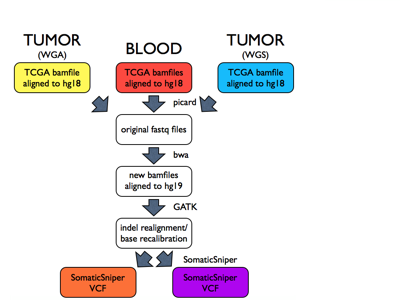
\includegraphics[scale=1.0]{data_processing_flowchart_2.png}
\caption{\textbf{Data processing flowchart.} For each of 55 patients, we began with a C484 tumor bamfile (WGS), a C282 tumor bamfile (WGA), and a normal bamfile, all aligned to hg18. For each bamfile, we used picard to regerate fastq files, bwa to realign the fastq files to hg19, GATK to recalibrate bases and indels, and SomaticSniper to call somatic mutations.}
\end{figure}

\begin{figure}
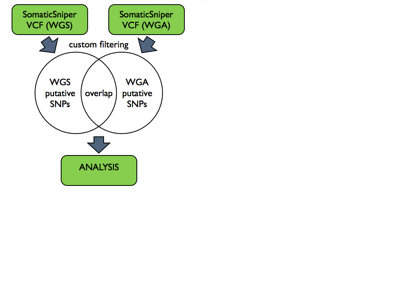
\includegraphics[scale=1.0]{overlap_explained.png}
\caption{\textbf{Overlap between WGS and WGA.} For each sample, we generated a SomaticSniper VCF with putative somatic mutations for each of two replicates. We took the overlap between the two lists for the most likely true positives.}
\end{figure}

\begin{figure}
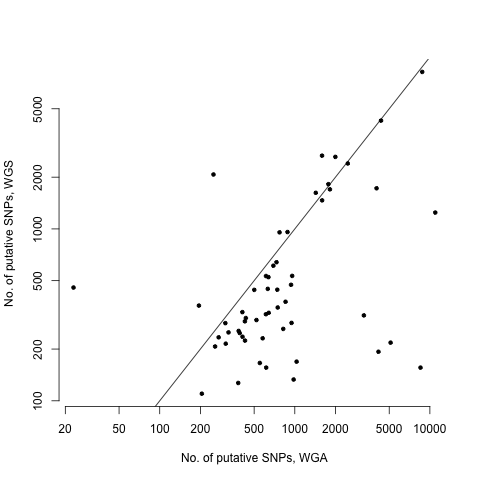
\includegraphics[scale=1.0]{C282_v_C484.png}
\caption{\textbf{Number of putative SNPs in WGS v. WGA, as called by SomaticSniper.} Each point is a patient. The line is y=x, so points falling below the line agree with the hypothesis that whole genome amplification makes more mutations in a sample.}
\end{figure}

\begin{figure}
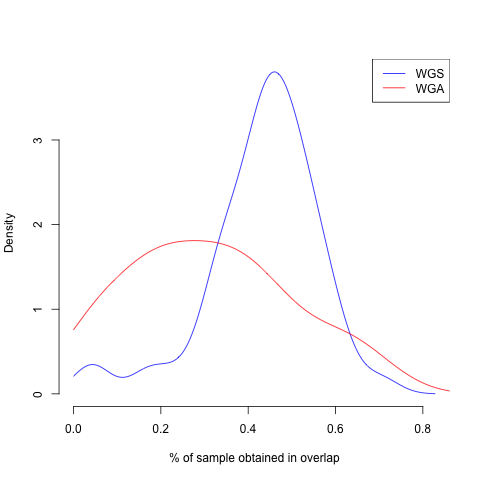
\includegraphics[scale=1.0]{unfiltered_overlap_WGS_WGA_together_densities.png}
\caption{\textbf{Density of percentage overlap between WGS and WGA samples.} This figure shows the density of the percentage of each WGS (blue) and WGA (red) sample that overlaps with the other sample from the same patient. The WGS distribution is higher and narrower, showing that the WGS samples overall have a higher percentage overlap than the WGA samples, and less range in this parameter. }
\end{figure}

\begin{figure}
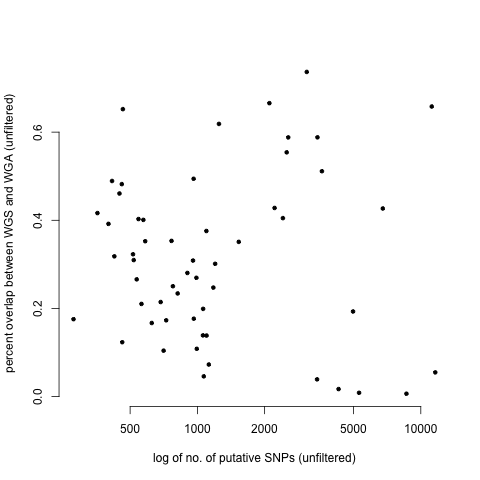
\includegraphics[scale=1.0]{unfiltered_total_muts_v_percent_overlap.png}
\caption{\textbf{Percent of WGS/WGA overlap versus (log) number of putative SNPs per sample.} Plot of the percentage of the WGA samples that overlaped with the corresponding WGS samples (as a measure of sample quality) against the total number of putative SNPs in the WGS sample.}
\end{figure}

\begin{figure}
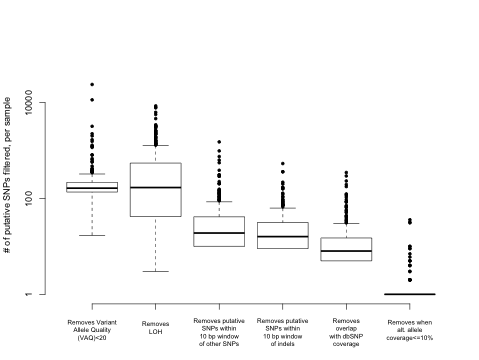
\includegraphics[scale=1.0]{boxplot_number_filtered.png}
\caption{\textbf{Number of putative SNPs removed by each of six filters.} The x-axis gives the name of those filters that removed putative SNPs, and the y-axis gives, on a log scale, the number of mutations removed by a given filter in a given sample. Filters removing LOH and low VAQ putative SNPs removed around 100-200 putative SNPs on average. Three other filters, removing overlap with dbSNP and putative SNPs close to other putaive mutations, removed on average ~50 mutations per sample.}
\end{figure}

\begin{figure}
% 379 samples, 311 pateints
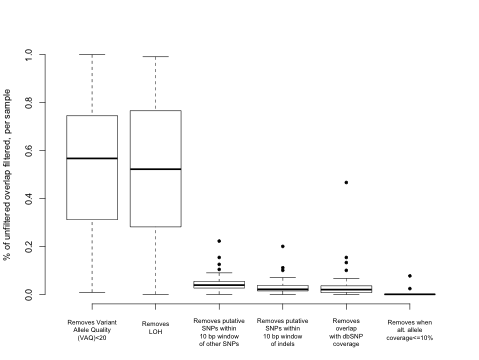
\includegraphics[scale=1.0]{boxplot_percent_overlap_filtered.png}
\caption{\textbf{Percentage of WGS/WGA overlap removed, by filter.} The x-axis describes the filters, and the y-axis gives the percentage of the WGS/WGA overlap removed by the filter, per sample. Filters removing LOH and putative SNPs with low VAQ removed a significant ercentage of the overlap; nothing else did.}
\end{figure}

% this is not the final path name, because this is not the final figure
\begin{figure}
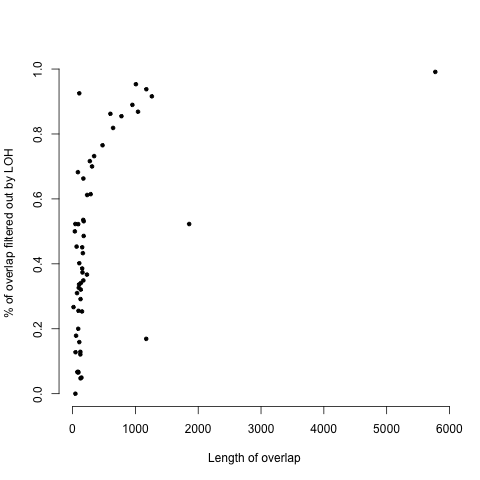
\includegraphics[scale=1.0]{./LOH_VAQ/LOH_all.png}
\caption{\textbf{Length of overlap of LOH segments.} As the length of the overlap between WGS and WGA increases (x-axis), the number of mutaitons filtered out by LOH increases. This is the opposite of the pattern observed in VAQ mutaitons (figure 6).}
\end{figure}

% this is not the final path name, because this is not the final figure
\begin{figure}
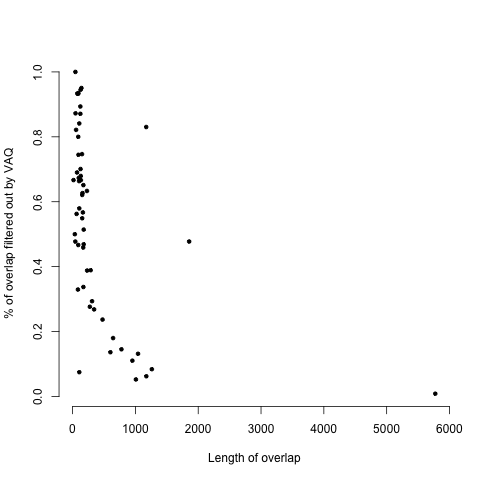
\includegraphics[scale=1.0]{./LOH_VAQ/VAQ_all.png}
\caption{ \textbf{Length of overlap of VAQ segments.} As the length of the overlap between WGS and WGA increases (x-axis), the number of mutaitons filtered out by VAQ decreases. This is the opposite of the pattern observed in LOH mutaitons (figure 5).}
\end{figure}

\bibliography{TCGA_bib}
\bibliographystyle{plain}

\end{document}

